\chapter{Objetivos}\label{cap.objetivos}
En este capitulo se presentaran los objetivos planteados para este proyecto y la metodología que se ha utilizado para alcanzarlos.

\section{Objetivos}
La principal meta de este trabajo será la de enriquecer con tecnologías web las herramientas robóticas existentes en la plataforma JdeRobot. Para alcanzar este objetivo, se ha dividido el trabajo en tres partes: 
\begin{itemize}
\item Modificar los tres visores elaboradas mediante tecnologías web existentes en la plataforma JdeRobot, CameraViewjs, KobukiViewerjs y UavViewerjs, para su utilización con el middleware ROS, además de ICE como hasta ahora. 
\item Creación mediante tecnologías web, de un nuevo visor, que permitirá la visualización de elementos 3D (puntos, líneas y modelos 3D) que utilizará como middleware de comunicación, ICE.
\item Elaborar un nuevo driver robótico utilizando tecnologías web, cuyo cometido será el de servidor de imágenes a los distintos visores existentes en JdeRobot.
\end{itemize}
Además, se ha utilizado el framework Electron en todos ellos para posibilitar que, además de usando un navegador, se puedan ejecutar como si de una aplicación de escritorio se tratase.

\section{Metodología}
La metodología elegida para la ejecución del trabajo ha sido el desarrollo en espiral. Se trata de uno de los modelos más utilizados en el desarrollo de software, y consiste en la realización de una serie de ciclos o iteraciones que se repiten en forma de espiral.
\begin{figure}[H]
  \begin{center}
    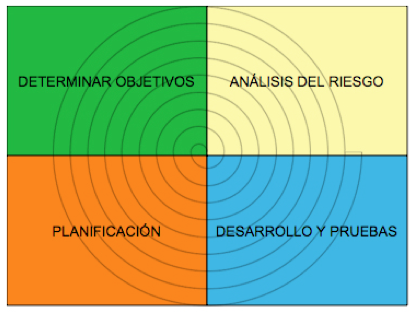
\includegraphics[width=0.8\textwidth]{figures/desarrolloespiral.png}
		\caption{Modelo de desarrollo en espiral}
		\label{fig.desarrolloespiral}
		\end{center}
\end{figure}
Cada iteración o ciclo esta formado por cuatro etapas.
\begin{enumerate}
\item Determinación de los objetivos a alcanzar para que el ciclo sea finalizado de manera exitosa.
\item Analizar los riegos que conlleva las elecciones tomadas para realizar el desarrollo, y establecer alternativas para solventar los posibles inconvenientes.
\item Desarrollar y probar los objetivos establecidos en la primera fase.
\item Planificar las siguientes etapas del proyecto, teniendo en cuenta los resultados obtenidos en esta interacción.
\end{enumerate}
De cara a poder llevar un mejor control del trabajo, se han tenido reuniones semanales con el tutor, en las que se marcaban los objetivos para la siguiente semana, se exponían dudas o posibles problemas  así como se establecen posibles alternativas, y se revisaba el trabajo previo. Con estas reuniones semanales se consigue tener flujo de trabajo constante y fluido, disminuyendo la posibilidad de quedar bloqueado en algún punto durante un largo periodo de tiempo.

Además, se ha elaborado un bitácora en la mediawiki\footnote{\url{https://jderobot.org/Rperez-tfg}} de JdeRobot, donde quede reflejado todos los progresos así como videos demostrativos de los avances. También se dispone de un repositorio en github\footnote{\url{https://github.com/RoboticsURJC-students/2017-tfg-roberto-perez}} donde se ha ido subiendo todo el código para su verificación y prueba por personas externas.

\section{Plan de Trabajo}
El plan de trabajo que se va a seguir es el siguiente:

\begin{enumerate}
\item Familiarización con las tecnologías que se van a utilizar en este trabajo: Lo primero que se realizará es entender el funcionamiento del framework Electron, la plataforma JdeRobot, el simulador Gazebo y los middleware ICE y ROS
\item Ampliación de las herramientas web existentes en la plataforma JdeRobot: Se adaptarán para ser usadas con Electron, y posteriormente se ampliarán, añadiendo la compatibilidad con el middleware ROS, de modo que puedan ser usadas con ambos middleware de comunicación.
\item Creación de un nuevo visor de objetos 3D: Primero se revisará el visor utilizado hasta ahora y desarrollado con C++. Una vez conocido su funcionamiento, se creará el nuevo visor 3D adaptando las conexiones ICE del visor antiguo para que funcionen con el nuevo. Finalmente, se ampliará el visor para que pueda mostrar más objetos de los que podía mostrar el visor antiguo.
\item Para terminar el trabajo, se implementará un nuevo driver que proporcionará un servidor de imágenes utilizando tecnologías web.
\end{enumerate}


